\documentclass{IEEEcsmag}

\usepackage[colorlinks,urlcolor=blue,linkcolor=blue,citecolor=blue]{hyperref}

\usepackage{color}
\usepackage{listings}
\usepackage{amssymb}
\definecolor{mygray}{rgb}{0.5,0.5,0.5}
\lstset{
numbers=left,
numbersep=5pt,
numberstyle=\tiny\color{mygray}
}
\jvol{XX}
\jnum{XX}
\paper{8}
\jmonth{May/June}
\jname{CiSE}
\pubyear{2019}
\newtheorem{theorem}{Theorem}
\newtheorem{lemma}{Lemma}

\setcounter{secnumdepth}{0}

\begin{document}

\sptitle{Department: Electronic Engineering}
\editor{Editor: Name, xxxx@email}

\title{Reproducing Scientific Experiment with Cloud DevOps}

\author{Feng Zhao}
\affil{Tsinghua University}

\author{Shaolun Huang}
\affil{Tsinghua University}

\author{\textbf{L}in Zhang}
\affil{Tsinghua University}

\markboth{Department Head}{Paper title}

\begin{abstract}
The reproducibility of scientific experiment is vital for the advancement of disciplines based on previous work. To achieve this goal, many researchers focus on complex methodology and self-invented tools which have difficulty in practical usage. In this article, we introduce the DevOps infrastructure from software engineering community and shows how DevOps can be used effectively to reproduce experiments for computer science related disciplines. DevOps can be enabled using freely available cloud computing machines for medium sized experiment and lab HPC environment for large scale computing, thus powering researchers to share their experiment result with others in a more reliable way.
\end{abstract}

\maketitle

\chapterinitial{THE INTRODUCTION} As the development of Big Data and Artificial Intelligence, computational scientific experiments encompass more disciplines but are much more complex than before. Training a useful AI model not only takes a long time but consumes huge memory and requires advanced computational device like GPU. Also, traditional simulation experiment like finite element analysis can be done on HPC cluster using more advanced parallel algorithms. There are also other emerging domains which are related to computational scientific experiment. These experiments require more dedicated toolchain, specific workflow, expensive and computational resources which put new challenge on experiment reproducibility.

To solve these issue, there are three kind of approaches: Tools, Platform and Methodology. Many tools \cite{greff2017sacred} are provided, which can capture the running environment information or storing the experiment result. These tools are valuable but may suffer from bad-maintainability and difficult configuration. Bad-maintainability originates from domain specific scientific software since their developers are not full-time software engineers. Experiment result storage requires the research to configure the database backend and the visualization needs some web technology. Also, most of these tools are not programming language neutral, which means researchers cannot use them in other programming languages. Still, the gain is more than the effort if more researchers use these tools to manage their experiment.

For platform solution, traditionally containerization is used. In recent years, it has been shown that cloud computing is suitable to be used for scientific research purpose \cite{Howe12}. However, configuration on cloud environment from scratch is difficult for unexperienced researches and it is better to use specific cloud service for research purpose. For example, we have Code Ocean or other commercial cloud systems \cite{perkel2018data}, which can tackle the reproducibility problem. The problem with such platform is that the free tier is mean and researchers probably are not willing to pay for much computational resource. Still, researchers can download the contents and run the replication locally and it is better than no code and no dataset are provided.

Methodology, or best practice in reproducibility usually discuss the general principals \cite{stodden2014best} or combines tools and platforms to explore the best practice \cite{QashaCW16}. Generally speaking, methodology is hard to follow as they tend to be ideal and the researchers may not be familiar with or have the ability to setup the toolchain used.  

Both the above three aspects have pros and cons for experiment reproducibility. Some researches seek more elegant solutions from software engineering community and give a try using Docker container for experiment reproducibility \cite{Boettiger15}.
Boettiger also mentioned the DevOps philosophy and acknowledged its limitations.
There have already been research projects which borrow the ideas of DevOps to develop domain specific infrastructure \cite{philips2019devops} or conduct sophisticated experiments \cite{chwalisz2019walker}. These previous research are valuable but they are limited to specific domain or tools and do not solve some critical problems:
\begin{enumerate}
\item The time, efforts and money researchers need to pay for such approach
\item High availability of the service used
\end{enumerate}

To be more specific, scientific researchers are not software engineering and many of them are not familiar with containerization technology. Either they have to spend much time and efforts to learn or pay money to use some user friendly 
cloud service (e.g. Code Ocean). Both are not satisfied for individual researchers. Also, newly developed platform such \texttt{Devops@mech} \cite{philips2019devops} or old services like Everest \cite{VOLKOV2017112} or VCR \cite{GavishD12} are hard to maintain since these services are provided by some laboratory and their users are very limited.

In this article, we will explore the solution from platform point of view. Our approach is not limited to a specific DevOps cloud service provider. Instead, we focus on the methodology and how to incorporate different tools within the model of DevOps for better experiment reproducibility. 
Also we will investigate the reproducibility problem in the domain of machine learning and graph computing and illustrate by concrete example how to use DevOps in these domains to help researchers be more productive and help others easier to follow their research. All too often, helping others actually helps yourself.

\section{INFRASTRUCTURE}
Originally, DevOps refers to the software engineering approach to automate the process of building and deploying software product, which is summarized by its another name ``Continuous Integration and Deployment (CICD)'' \cite{bass2015devops}. 
DevOps service (server) can be self-hosted or centrally hosted. DevOps server is quite complex and self-hosted solution is not suitable for sharing results with others. Besides, self-hosted computing agent (client) can be used if public provided agent is not suitable to reproduce the experiment. In this article, we only consider cloud hosted DevOps solution for experiment reproducibility.

There are some similarities between cloud DevOps and Everest infrastructure \cite{GavishD12} . Both of cloud DevOps and Everest allow dynamic provision of computing resources from public cloud service provider and support computing resources attached by users. The computation can be trigger by user click the button via web interface. But DevOps cloud service is superior than Everest not only because more flexible configuration and high availability but also because the former is easier to use. DevOps cloud service has complete documentation, FAQ, community support and most importantly developer first philosophy while self-made platform lacks.  From the workflow management point of view, cloud DevOps is similar to Pegasus system \cite{Pegasus}. While the latter is more suitable for large scale distributed computing management, cloud DevOps is scalable and covers the need from small experiment to large scale experiment as well.

% notebook approach 
There are many freely available cloud DevOps service for open source project which greatly powers individual developers and open source community. {\bf Table} \ref{tab1} gives some famous providers, with the list of their features and the privileges if the researchers make their source code open.

\begin{table}
\caption{Comparison of Cloud DevOps provider (until 2019)}
\label{table}
\small
\begin{tabular*}{17.5pc}{@{}|p{39pt}|p{73pt}<{\raggedright}|p{60pt}<{\raggedright}|@{}}
\hline
Name& 
Features& 
Open Source Project Privilege\\
\hline
AppVeyor& Windows \& Linux support & unlimited public projects; 1 concurrent job with unlimited time; 5 self-hosted jobs
 \\
 \hline
 Azure pipelines & cross-platform, Windows \& Linux docker support, predefined task & 10 hosted job with unlimited time; unlimited self-hosted CICD
 \\
 \hline
   CircleCI & cross-platform, Linux docker support & 4 Linux containers with no time limit  \\
 \hline
GitLab CICD& Linux docker support & free to use

\\
\hline
GitHub Actions& cross-platform,Linux docker support, programming language support
& unlimited projects and running time
\\
\hline
Travis& 
cross-platform; multiple programming language support; various deployment choice
& 2 concurrent jobs; unlimited minutes
\\
\hline
\end{tabular*}
\label{tab1}
\end{table}

We call a DevOps infrastructure cross-platform if it supports Windows, MacOS and Linux (usually Ubuntu) Operating Systems.
Cross-platform is an important topic in software engineering. For scientific community, most research experiments can only be reproduced on specific version of one Operating System. This is OK since researchers are not specialist on software engineering and have not machines of other Operating Systems or spare time to make their code run on different platforms. Nowadays, things are different. DevOps provides easy configuration for different environments and researchers are encouraged to test their code on them without learning too much new knowledge and spending too much time. Researchers can first choose the most similar environment on the cloud to their local development environment and make the cloud version works. We believe it is beneficial if newly developed algorithms and experiments can be run on more platforms. 

DevOps or its equivalent term CICD consists of two parts: environment specification and pipeline description. 
Both of them are described in a configuration file with \texttt{YAML} format. This is adopted by all cloud DevOps provider though the content schema differs a little. Below we give a short introduction of the two aspects of Cloud DevOps configuration:
\subsection{Choosing Environment for Agent}
For the environment configuration part, users choose the actually running time of their code. Usually, it is predefined combination of the following items:
\begin{enumerate}
\item normal operating system or virtualized image.
\item splitting different phases or put everything in one place.
\item public cloud service or local runner.
\item programming language and version.
\end{enumerate}

For example, on Travis users can have Ubuntu 16.04 \texttt{Python 3.6} environment by simple requires it in the following way:
\begin{lstlisting}[caption={environment configuration}]
os: linux
dist: xenial
language: python
python: 3.7
\end{lstlisting}

In this configuration, we use normal OS provided by cloud service. Under such environment, \texttt{python} command is actually 3.6 from the official release.
Such shortcut makes install dependency in later workflow management much easier as we do not need to install the interpreter and configure the environment variable manually.

It should be noticed that not all DevOps infrastructure supports every combination of the above. For example, many platforms do not support connecting the local runner to the cloud or only support certain environment combination. Details about environment configuration can be obtained from the official documentation of the provider.

Besides normal operating system environment, many DevOps infrastructures support Docker containers or the researches can run their own containers (whether it is Docker based, Singularity based or other virtual machines) in their self-hosted agent. Virtualization is better than normal OS for experiment reproducibility but it is also more complex to configure. We do not elaborate such workflow but we encourage the researchers to have a try.

The system diagram in \textbf{Figure} \ref{fig:principal} shows the interaction between the agent, the cloud DevOps server and the source code repository. 
This is a typical use cases when DevOps incorporates the source code version control. The advantage is that each log has a unique identifier associated with the commit hash of the source. By inspecting the public available log and the source code at specific commit stage, others can reproduce the same result using public available build machine or on local workstations.

\begin{figure}[!ht]
\centerline{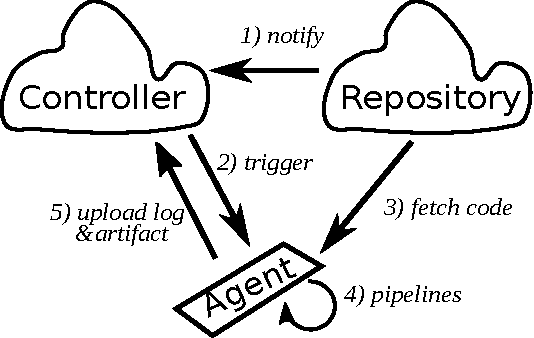
\includegraphics[width=18.5pc]{principal.pdf}}
\caption{Interaction of DevOps server with agent and source code repository}\label{fig:principal}
\end{figure}

Though we can use the cloud computing resources for unlimited time, the parallel ability is restricted and special computing device (like GPU) or infrastructure (MPI) is missing. The ability to use self-hosted environment is important to run complex scientific experiment. Fortunately, many cloud DevOps service provides the local agent option to make it possible. By installing a client software, it is possible to empower the advantages of cloud DevOps without losing the computing ability of lab servers. 
\subsection{workflow description}
In this step, users should determine how to execute their code sequentially. The basic workflow can be summarized in \textbf{Figure} \ref{fig:cicdworkflow}.

\begin{figure}[!ht]
\centerline{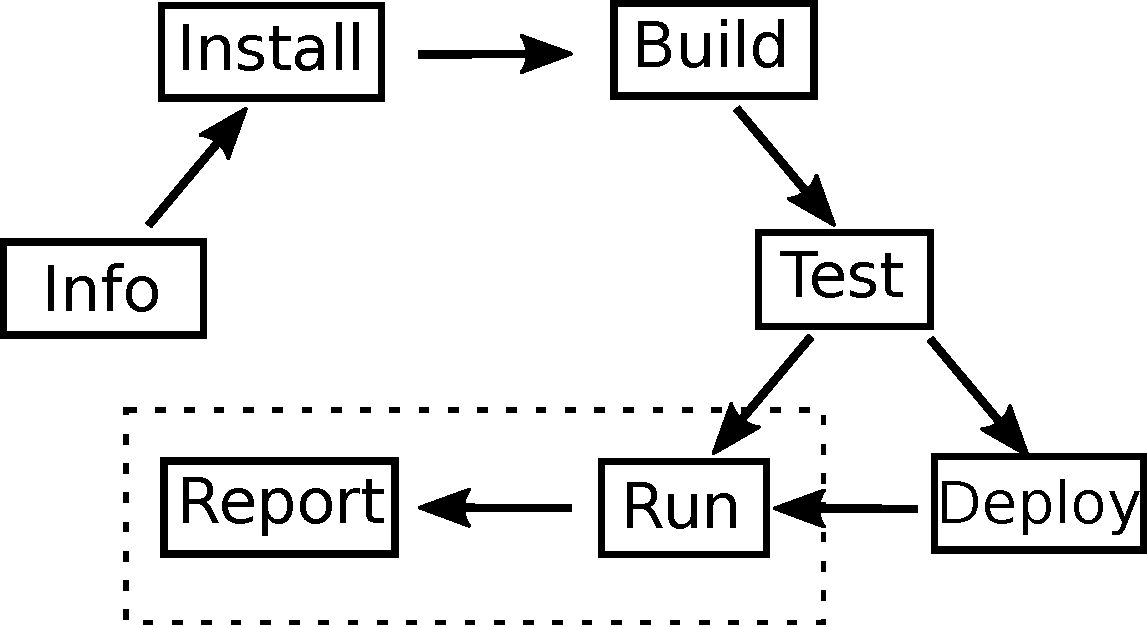
\includegraphics[width=18.5pc]{workflow.pdf}}
\caption{CICD pipeline illustration. The steps within blue boxes are specific stages for scientific experiments. }\label{fig:cicdworkflow}
\end{figure}
%\item build artifact or have deployment stage
%\item build artifact or have deployment stage

The first few steps are common. We need to capture enough information of the running machine and install necessary software dependencies. Then we build our source code to binary executable and run some test to verify whether it works for simple cases. In software engineering community, DevOps ends with the deployment step. But for scientific computing community, the story just begins after packing your method or algorithm implementation. Therefore, we use blue boxes to emphasis the unique steps for scientific experiment in DevOps infrastructure. After the experiment finishes, the result needs to be collected and further processed and we call this step Report.

For the Info step, it is automatically done by DevOps server. For other steps, shell scripts are used to tell the running machine how to install, build etc. Suppose a researcher writes his experiment code using Python programming language, then he can write his workflow as follows:
\begin{lstlisting}[caption={workflow description}, label={lst:wd}]
install: 
  - pip install -r requirements.txt
script: # run experiment
  - python main.py
\end{lstlisting}

In the above workflow description, Build, Test and Deploy steps are omitted. This is common for many researchers, especially when interpreted language is used. This is OK as long as the experiment results are all right. Still, it is better to do some test and do some deployment task. Deployment makes other researchers easier to compare their results with your method without copying your code into their code repository.

%Also, DevOps can be customized by self hosting the server in the laboratory or using local runner on workstation or HPC cluster.
Since the infrastructure of cloud DevOps service is transparent to all users and the mechanism of it is totally determined by configuration file and specific commit of source code. Other researchers can trust the output logs DevOps as evidence of experiment reproducibility. Rerunning the code is also very easier, just use the same service provider and the code can be run under a different account. We acknowledge that this convenience is not applicable to self-hosted agent. For self-hosted agent usually the environment configuration part is not written in a file but determined by which type of agent used. Virtualization is a solution to such a program but compared with building complex virtual image and starting it locally, we encourage the research to run a partial and small scale experiment on public DevOps server and run their full experiment on self-hosted server using the same code base. The log files uploaded from self-hosted agent can demonstrate the reproducibility to some extent.

\section{CASE STUDIES}
In the previous section, we briefly overview the common practice in DevOps and how it can be related with scientific experiment reproducibility. Different domains 

\subsection{Machine Learning}
Experiment Reproducibility is argued in ML community \cite{kegl2018ramp}. Reproducibility in ML Workshop discussed the problem from different perspective. Researchers can try more dedicated tools and contribute to their development. But before that, it is preferable to use more simple and flexible approach to resolve the reproducibility problem. In this subsection, we mention some aspects of reproducibility using examples in the domain of machine learning.

The workflow shown in Fig \ref{fig:cicdworkflow} can be further decomposed into two phases:
Algorithm library build phase and experiment executable phase. The output of the first phase is the reusable library which is one of input to the second phase. Using DevOps in the first phase is nearly identical to the development of other softwares. 
The reusable library can be deployed to public available package repository. For example, in Python programming language, it is \url{pypi.org}. {\bf Table} \ref{tab:deploy} shows the deployment result to pypi made by an independent researcher using DevOps. 
\begin{table}
\centering
\begin{tabular}{|c|c|c|c|}
\hline
OS & py3.6 & py3.7  & provider badge\\
\hline
Windows & \checkmark & \checkmark  & 
\includegraphics[width=2cm]{./appveyor.pdf}\\ 
\hline
MacOS & \checkmark & \checkmark & 
\includegraphics[width=2cm]{./travis.pdf}\\ 
\hline
ManyLinux & \checkmark & \checkmark & same as above \\
\hline
\end{tabular}
\caption{cross-platform deployment matrix of pspartition algorithm used in scientific experiment}\label{tab:deploy}
\end{table}

This deployment is cross-platform and supports different version of Python\footnote{For Python extension package, we need to package binary executable.} For the second stage, we can just install the deployed package and run the actual experiment. The specification can be the same with Listing \ref{lst:wd}. In the requirements file, put your algorithm package name and others in it. In our practice (info-detection-experiment), we use sacred tool \cite{greff2017sacred} to manage the experiment logic and each running log can be checked out publicly on the DevOps provider we used (Travis).


% another experiment, focues on data fetching and model training and saving

\subsection{HPC}
Experiment Reproducibility on high performance cluster has extra difficulty because of its parallelism. Singularity is a virtualization solution targeted at such case. % citation needed
Also, other dedicated tools can be used like Guix, which powers non-admin to manage and share their package on HPC \cite{courtes2015reproducible}. These prior work can be combined with the power of DevOps service and strength the reproducibility of HPC experiment. Since the general workflow for users of HPC is they submit a job from head node using a workload manager, the same job can be submitted by self-hosted DevOps agent, which is illustrated by {\bf Figure} \ref{fig:selfhosted}. Using agent to submit job has extra advantages that the running log are preserved in a continuous way without messing things up. Generally only the second stage in Figure \ref{fig:cicdworkflow}
is executed in self-hosted agent. Going through the whole pipeline costs extra time but makes the experiment more reliable.

\begin{figure}[!ht]
\centerline{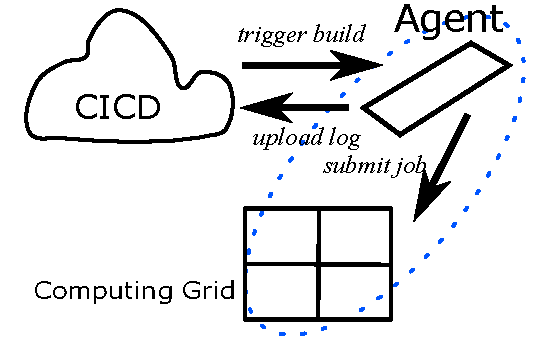
\includegraphics[width=18.5pc]{self-hosted.pdf}}
\caption{Using self-hosted HPC to connect DevOps server. The blue ellipse part is self-hosted resources.}\label{fig:selfhosted}
\end{figure}

We give a simple experiment which uses OpenMP to parallel the program. The complexity depends on the input data. For two kinds of input data, the detail is shown in {\bf Table} \ref{tab:time}.
\begin{table}
\centering
\begin{tabular}{|c|p{1.5cm}|p{1.5cm}|}
\hline
Data Size & 527 MB & 2.0 GB\\
\hline
Data Source & Git LFS & HPC Storage Node \\
\hline
Platform & Travis Public Agent & HPC Computing Node \\
\hline
CPU Core & 2 & 32  \\ 
\hline
Peak Memory  & 3.1 GB  & 17.9 GB\\ 
\hline
Time & 4.3 Minutes & 10.5 Hours \\
\hline
\end{tabular}
\caption{Program running time and its requirements on public server and self-hosted agent}\label{tab:time}
\end{table}

The program is compiled from the same source code. We run a medium-sized experiment on the freely-available cloud server and the full experiment is run on self-hosted agent. These combination increases the reproducibility of the project.

Special consideration of the data is needed. Since fetching data from external web is time-consuming and wastes bandwidth, we can store the data using cache feature in cloud server. For self-hosted case, storing data is much more obvious but the arbitrary path may let the experiment hard to follow. Also, it is not transparent if loading data directly from self-hosted disk because others do not know whether it is original data or not. Checksum is a good way to guarantee this. We recommend researchers to verify the checksums of the data to the precomputed ground truth whether the data is downloaded freshly or loaded from cache. By guaranteeing the data integrity can the experiment be more rigorous and convincing.

% introduce run the time complexity experiment on the self-hosted server

% graph computation experiment, focues on parallel power and HPC cluster usage

\section{CONCLUSION}
DevOps infrastructure is actively maintained by software engineering community and evolves towards better usability. It will be beneficial for scientists if they could incorporate DevOps into their daily research. DevOps can improve the experiment reproducibility if medium-sized experiments can be run directly on public DevOps service and complete logs are available for large-scale experiments. Currently, it is unknown the accessibility of DevOps by scientific community beyond scientific software development. Since DevOps is easily configurable and compatible with existing tools, we believe it will sweep more disciplines in the future.

\section{ACKNOWLEDGMENT}

This work is supported by the Natural Science Foundation of China 61807021, Shenzhen Science and Technology Research and Development Funds (JCYJ20170818094022586), and Innovation and entrepreneurship project for overseas high-level talents of Shenzhen (KQJSCX20180327144037831).


\bibliographystyle{IEEEtran}
\bibliography{exportlist}



\begin{IEEEbiography}{Feng Zhao}{\,} is
currently with Tsinghua University, PR. China. He received the B.S. degree and is pursing Ph.D degree at Department of Electronic Engineering. His research interest focus on machine learning, graph computing and scientific computing. Contact him at zhaof17@mails.tsinghua.edu.cn.
\end{IEEEbiography}

\begin{IEEEbiography}{Shaolun Huang,}{\,}is a Professor with Tsinghua-Berkley Shenzhen Institute. Contact him at shaolun.huang@sz.tsinghua.edu.cn.
\end{IEEEbiography}

\begin{IEEEbiography}{Lin Zhang,}{\,}is a Professor with Tsinghua Shenzhen International Graduate School. Contact him at linzhang@tsinghua.edu.cn.
\end{IEEEbiography}

\end{document}

